\chapter{Introduction}\label{sec:introduction}
	
		Building simulation are widely used for different purposes such as to benchmark buildings or to evaluate energy demands and indoor thermal comforts. However, due to a number of factors, there are deviations between calculated  and measurement values, which is called \textbf{performance gap}. Previous studies which used a standardized method \textbf{SIA 180/1} to calculate the heating demand of several buildings observed considerably large performance gaps in uninsulated buildings as shown in \ref{fig:SIA380PG} \cite{SIAPreviousreport}. It is believed that part of the problem come from a non-accurate calculation method or non-realistic assumptions to some building parameters and outdoor environment \cite{SIAPreviousreport}. \\
	
	
		Therefore, the purpose of this thesis is to find out the main causes of the performance gap in uninsulated buildings, as well as the most influential factors in building simulation. In addition, this thesis also aims to investigate how the resulting energy demand variations affect the performance gap.\\

	
		Two uninsulated buildings, one residential and one office buildings, are carefully modeled and analyzed using different approaches including static calculation (SIA 180/1) and dynamic simulation (EnergyPlus). The buildings is firstly calibrated to match the historical measurement, then building parameters are modified and the most influential factors can be discovered.\\

			\begin{figure}[h!]
			\centering
			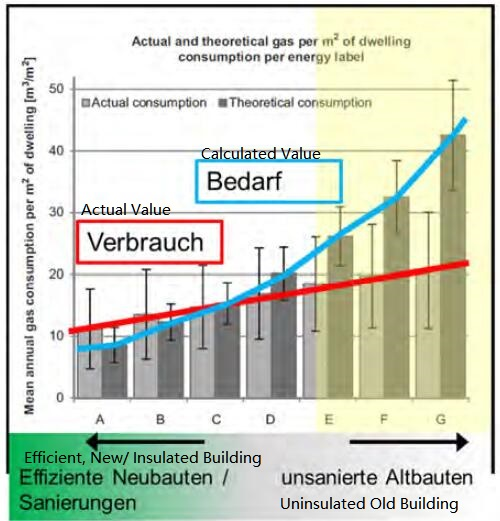
\includegraphics[scale=0.65]{Figure/SIA380Issue.jpg}
			\caption{SIA380/1 Calculation Performance Gap Indicator \cite{SIAPreviousreport}}
			\label{fig:SIA380PG}
			\end{figure}

